\documentclass[a4paper]{article}

\usepackage[portuguese,english]{babel}
\usepackage[utf8]{inputenc}
\usepackage[T1]{fontenc}

\newcommand{\documentTitle}{Data Analysis and Transformation \\ TP1: Fundamentals of Signals and Systems}
\newcommand{\pdfTitle}{[ATD] TP1: Fundamentals of Signals and Systems}
\newcommand{\documentAuthors}{José Ribeiro (2008112181, jbaia@student.dei.uc.pt) \\ Pedro Magalhães (2009117002, pjrosa@student.dei.uc.pt)}

\title{\documentTitle}
\author{\documentAuthors}

\usepackage{hyperref}
\hypersetup{
	pdftitle = \pdfTitle
	,pdfauthor = \documentAuthors
	,pdfsubject = {Data Analysis and Transformation}
	,pdfkeywords = {Data Analysis and Transformation} {Signal Processing}
	,pdfborder = {0 0 0}
}

%\usepackage{subfig}
%\usepackage{amsmath}
%\usepackage{array}
\usepackage{anysize}
\usepackage{lscape}
\usepackage{amsmath}
\usepackage{graphicx}
\usepackage{caption}
\usepackage{amssymb}
%\usepackage[pdftex]{graphicx}
%\usepackage[table]{xcolor}

\hyphenation{}

\marginsize{2.7cm}{2.7cm}{3cm}{3cm}

\makeatletter

\begin{document}
\maketitle
\cleardoublepage

\tableofcontents
\cleardoublepage

\setlength{\parindent}{1cm}
\setlength{\parskip}{0.3cm}

\section{Exercise 1}
\subsection{Exercise 1.1}
\noindent Após substituição das variáveis pelo número de grupo, obtém-se a seguinte expressão:
\begin{equation}
	y[n] = 0.3137 \, x[n - 3] - 0.1537 \, x[n - 5] + 2.3 \, y[n - 1] - 1.74 \, y[n - 2] + 0.432 \, y[n - 3] \\
\end{equation}

\noindent A partir da expressão obtém-se
\begin{equation}
	y[n] - 2.3 \, y[n - 1] + 1.74 \, y[n - 2] - 0.432 \, y[n - 3] = 0.3137 \, x[n - 3] - 0.1537 \, x[n - 5] \\
\end{equation}

\noindent Aplicada a Transformada Z em ambos os lados da expressão

\begin{equation}
	\mathcal{Z}(y[n] - 2.3 \, y[n - 1] + 1.74 \, y[n - 2] - 0.432 \, y[n - 3]) = \mathcal{Z}(0.3137 \, x[n - 3] - 0.1537 \, x[n - 5])
\end{equation}

\noindent é possível obter-se a Função de Transferência do Sistema na forma polinomial.

\noindent Dado que
\begin{eqnarray}
	G(z) & = & H(z)|_{\text{condições iniciais nulas}} \\
		 & = & \mathcal{Z}\{h[n]\} \\
		 & = & \frac{Y(z)}{X(z)}
\end{eqnarray}

\noindent tem-se que
\begin{eqnarray}
	&\mathcal{Z}\{y[n] - 2.3 \, y[n - 1] + 1.74 \, y[n - 2] - 0.432 \, y[n - 3]\} = \mathcal{Z}\{0.3137 \, x[n - 3] - 0.1537 \, x[n - 5]\} \\
	&Y(z) - 2.3 \, z^{-1} \, Y(z) + 1.74 \, z^{-2} \, Y(z) - 0.432 \, z^{-3} \, Y(z) = 0.3137 \, z^{-3} \, X(z) - 0.1537 \, z^{-5} \, X(z) \\
	&Y(z) (1 - 2.3 \, z^{-1} + 1.74 \, z^{-2} - 0.432 \, z^{-3}) = X(z)(0.3137 \, z^{-3} - 0.1537 \, z^{-5}) \\
	&\frac{Y(z)}{X(z)} = \frac{0.3137 \, z^{-3} - 0.1537 \, z^{-5}}{1 - 2.3 \, z^{-1} + 1.74 \, z^{-2} - 0.432 \, z^{-3}} \\
	&\frac{Y(z)}{X(z)} = \frac{z^{5} \, (0.3137 \, z^{-3} - 0.1537 \, z^{-5})}{z^{5} \, (1 - 2.3 \, z^{-1} + 1.74 \, z^{-2} - 0.432 \, z^{-3})} \\
	&\frac{Y(z)}{X(z)} = \frac{0.3137 \, z^{2} - 0.1537}{z^{5} - 2.3 \, z^{4} + 1.74 \, z^{3} - 0.432 \, z^{2}}
\end{eqnarray}

\noindent pelo que se obtém que
\begin{equation}
	\label{eq:tf}
	G(z) = \frac{0.3137 \, z^{2} - 0.1537}{z^{5} - 2.3 \, z^{4} + 1.74 \, z^{3} - 0.432 \, z^{2}}
\end{equation}

\subsection{Exercise 1.2}
\subsubsection{Exercise 1.2.1/1.2.2}
\noindent A localização dos zeros e pólos de um sistema no plano $Z$ fornece informações relativamente à estabilidade de um sistema. A partir da função de transferência (equação \ref{eq:tf}), é possível obter os zeros e pólos calculando os zeros do numerador e do denonimador, respectivamente. Como tal, obtiveram-se os zeros $\pm 0.7$ e os pólos $[0, 0, 0.6, 0.8, 0.9]$.

\noindent De seguida apresenta-se a representação dos zeros e pólos no plano $Z$.
\begin{center}
	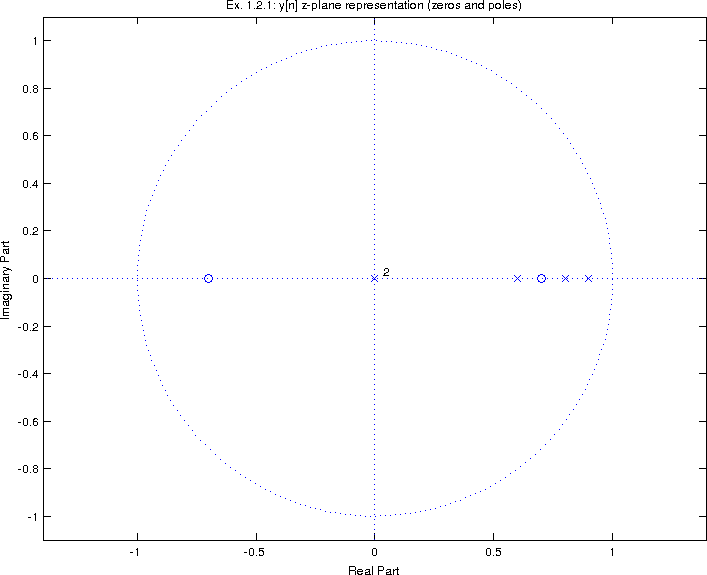
\includegraphics[width=0.65\textwidth]{images/ex1_2_1.png}
	\captionof{figure}{$y[n]$ z-plane representation (zeros and poles).}
	\label{fig:ex1_2_1_zplane}
\end{center}

\noindent Como se pode observar, todos os pólos e raízes estão contidos no círculo de raio unitário. Como tal, este sistema é \textbf{estável}.

\subsubsection{Exercise 1.2.3}
\label{subsubsec:ex1_2_3}
\noindent Dado que assumimos que
\begin{equation}
	G(z) = H(z)|_{\text{condições iniciais nulas}} \\
\end{equation}

\noindent é possível obter a expressão da resposta a impulso do sistema, $h[n]$, válida para $n \ge 0$, aplicando à função de transferência anteriormente obtida a Transformada Inversa de $Z$ ($\mathcal{Z}^{-1}$). Utilizando a função \texttt{iztrans} do \texttt{MATLAB} obteve-se a expressão
\begin{equation}
	h[n] = \mathcal{Z}^{-1}\{G(z)\} = \frac{44573}{31104} \, \delta[n - 1] + \frac{1537}{4320} \, \delta[n - 2] - \frac{1274 \, (\frac{3}{5}) ^ n}{405} - \frac{11767 \, (\frac{4}{5}) ^ n}{2560} + \frac{100397 \, (\frac{9}{10}) ^ n}{21870} + \frac{17644573}{5598720} \, \delta[n]
\end{equation}

\subsubsection{Exercise 1.2.4}
\noindent Em seguida apresenta-se a resposta a impulso do sistema, segundo a expressão obtida em \emph{\nameref{subsubsec:ex1_2_3}} (azul) e segundo as funções do \texttt{MATLAB} \texttt{impz} (vermelho) e \texttt{dimpulse} (verde).

\begin{center}
	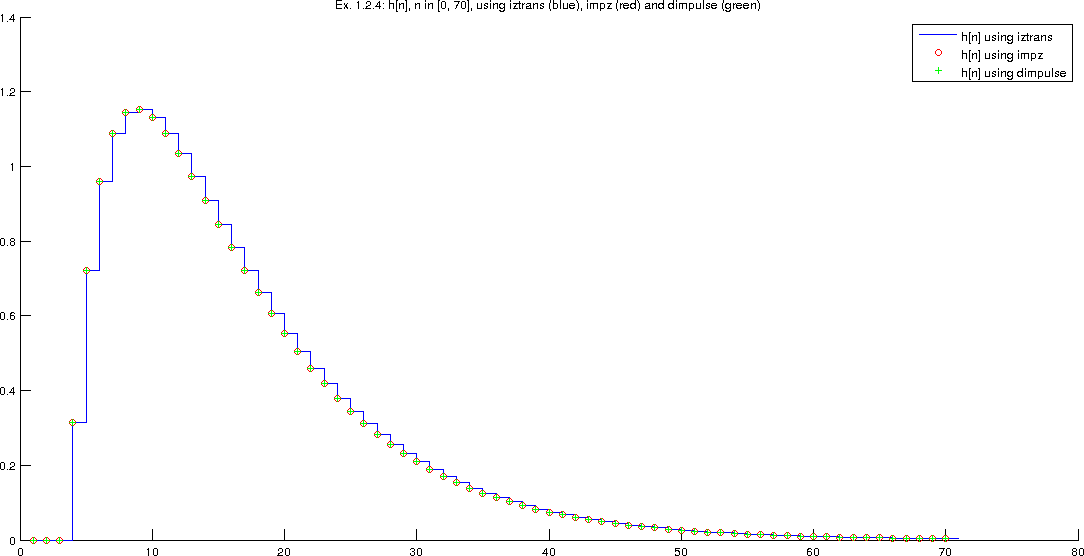
\includegraphics[width=0.70\textwidth]{images/ex1_2_4.png}
	\captionof{figure}{$h[n]$, $n \in [0, 70]$, using \texttt{iztrans} (blue), \texttt{impz} (red) and \texttt{dimpulse} (green).}
	\label{fig:ex1_2_4_zplane}
\end{center}

\subsubsection{Exercise 1.2.5}
\label{subsubsec:ex_1_2_5}
\noindent Considerando que é conhecida a expressão de $H(z)$, é possível obter a resposta do sistema ao degrau unitário ($u[n]$) usando a igualdade
\begin{equation}
	\label{eq:ex_1_2_5_system_response}
	Y(z) = X(z) \, H(z)
\end{equation}

\noindent onde $X(z)$ deverá ser substituída por $U(z)$, Transformada de $Z$ de $u[n]$. $U(z)$ é dada por
\begin{equation}
	\label{eq:ex_1_2_5_unit_step_response_ztrans}
	U(z) = \frac{1}{1 - z^{-1}}
\end{equation}

\noindent O resultado desse produto dará a Transformada de $Z$ da resposta do sistema ao degrau unitário. Isto é,
\begin{eqnarray}
	\label{eqnarr:ex_1_2_5_unit_step_response_ztrans_replace}
	Y(z) & = & U(z) \, H(z) \\
	& = & \frac{1}{1 - z^{-1}} \, \frac{0.3137 \, z^{2} - 0.1537}{z^{5} - 2.3 \, z^{4} + 1.74 \, z^{3} - 0.432 \, z^{2}}
\end{eqnarray}

\noindent Como queremos a expressão da resposta do sistema, tem de ser aplicada a Transformada Inversa de $Z$, $\mathcal{Z}^{-1}$. Utilizando a função \texttt{iztrans} do \texttt{MATLAB}:
\begin{equation}
	\label{eq:ex_1_2_5_unit_step_response}
	y[n] = \mathcal{Z}^{-1}\{Y(z)\} = \frac{637 \, \left(\frac{3}{5}\right)^n}{135} - \frac{1537 \, \delta[n - 1]}{4320} + \frac{11767 \, \left(\frac{4}{5}\right)^n}{640} - \frac{100397 \, \left(\frac{9}{10}\right)^n}{2430} - \frac{278197 \, \delta[n]}{155520} + 20
\end{equation}

\subsubsection{Exercise 1.2.6}
\noindent Em seguida apresenta-se a resposta do sistema ao degrau unitário, segundo a equação (\ref{eq:ex_1_2_5_unit_step_response}) (azul) e segundo a função do \texttt{MATLAB} \texttt{dstep} (vermelho).
\begin{center}
	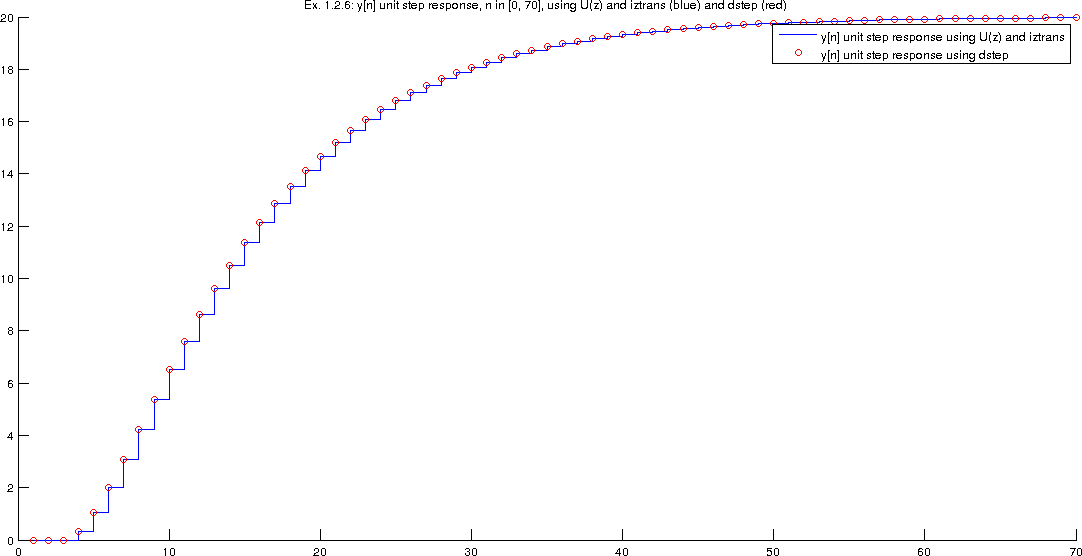
\includegraphics[width=0.70\textwidth]{images/ex1_2_6.png}
	\captionof{figure}{$y[n]$ unit step response, $n \in [0, 70]$, using $U(z)$ and \texttt{iztrans} (blue) and \texttt{dstep} (red).}
	\label{fig:ex1_2_6}
\end{center}

\subsubsection{Exercise 1.2.7}
\noindent Para computar a resposta do sistema para uma dada entrada, considera-se que é dada segundo o formato simbólico do \texttt{MATLAB}. Calcula-se a sua Transformada de $Z$, que por convolução com a função de transferência, origina a Transformada de $Z$ dessa resposta. Após isso, em semelhança a \nameref{subsubsec:ex_1_2_5}, é aplicada a Transformada Inversa de $Z$ ao resultado, o que origina a expressão da resposta do sistema para uma dada entrada.

\subsubsection{Exercise 1.2.8}
\noindent Em seguida apresenta-se a resposta do sistema para uma dada entrada, segundo a equação (\ref{eq:ex_1_2_5_system_response}) (após a aplicação da Transformada de $Z$ sobre essa entrada) (azul) e segundo as funções do \texttt{MATLAB} \texttt{filter} (vermelho) and \texttt{dlsim} (verde).
\begin{center}
	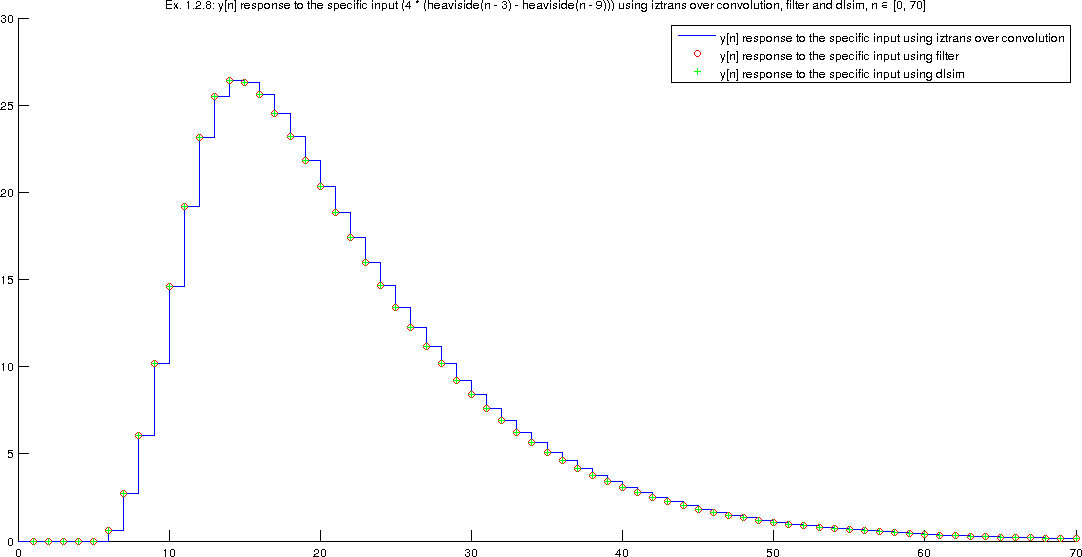
\includegraphics[width=0.70\textwidth]{images/ex1_2_8.png}
	\captionof{figure}{$y[n]$ response to the specific input (\texttt{4 * (heaviside(n - 3) - heaviside(n - 9))} using \texttt{iztrans} over convolution (blue), \texttt{filter} (red) and \texttt{dlsim} (green), $n \in [0, 70]$}
	\label{fig:ex1_2_8}
\end{center}

\subsubsection{Exercise 1.2.9}
\noindent Em seguida apresentam-se os gráficos da resposta do sistema em frequência, $H(\Omega)$, para $\Omega \in [0, \pi] rad$, em amplitude (em cima, em decibéis ($dB$)) e em fase (em baixo, em graus).
\begin{center}
	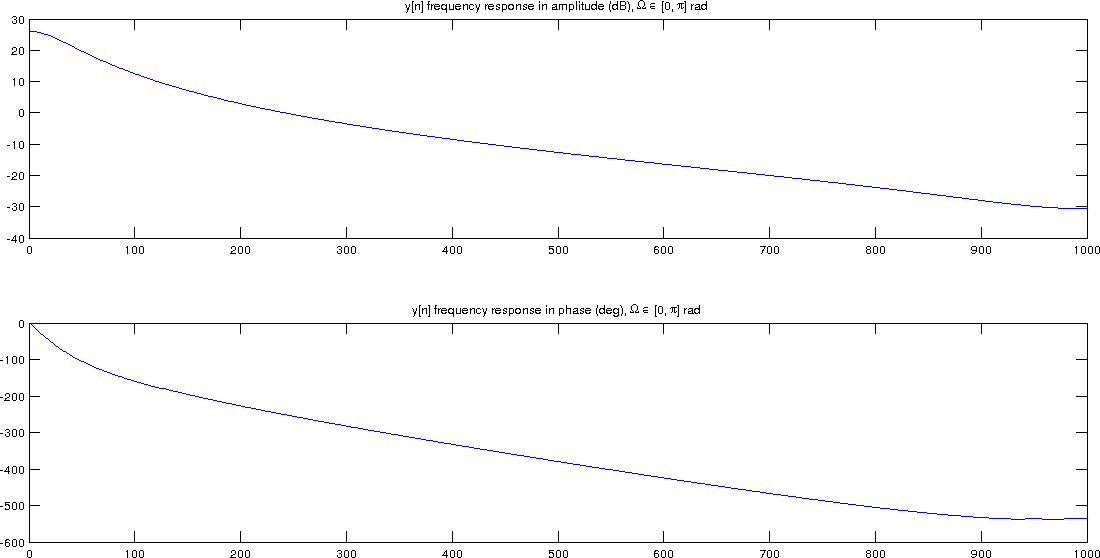
\includegraphics[width=0.70\textwidth]{images/ex1_2_9.png}
	\captionof{figure}{$y[n]$ frequency response in amplitude (dB) and phase (deg), $\Omega \in [0, \pi] \, rad$.}
	\label{fig:ex1_2_9}
\end{center}

\subsubsection{Exercise 1.2.10}
\noindent Dada a equação do Teorema do Valor Final
\begin{equation}
	y[\infty] = \lim_{z \to 1} \, (1 - z^{-1}) \, Y(z)
\end{equation}

\noindent e substituindo Y(z) pela expressão obtida na equação (\ref{eqnarr:ex_1_2_5_unit_step_response_ztrans_replace}), assumindo a igualdade da equação (\ref{eq:ex_1_2_5_unit_step_response_ztrans}) obtém-se que
\begin{eqnarray}
	y[\infty] & = & \lim_{z \to 1} \, (1 - z^{-1}) \, \frac{1}{1 - z^{-1}} \, H(z) \\
	& = & \lim_{z \to 1} \, H(z)
\end{eqnarray}

\noindent Após a substituição pela função de transferência (assumindo condições iniciais nulas), obtém-se que
\begin{eqnarray}
	\lim_{z \to 1} \, H(z) & = & \frac{0.3137 \, z^{2} - 0.1537}{z^{5} - 2.3 \, z^{4} + 1.74 \, z^{3} - 0.432 \, z^{2}} \\
	& = & \frac{0.3137 * 1^{2} - 0.1537}{1^{5} - 2.3 * 1^{4} + 1.74 * 1^{3} - 0.432 * 1^{2}} \\
	& = & \frac{0.3137 - 0.1537}{1 - 2.3 + 1.74 - 0.432} \\
	& = & \frac{0.16}{0.008} \\
	& = & 20
\end{eqnarray}

\noindent Utilizando a equação \ref{eq:ex_1_2_5_unit_step_response}, obtida em \emph{\nameref{subsubsec:ex_1_2_5}}, obtém-se esse mesmo valor:
\begin{eqnarray}
	y[\infty] & = & \lim_{n \to \infty} \, \frac{637 \, \left(\frac{3}{5}\right)^n}{135} - \frac{1537 \, \delta[n - 1]}{4320} + \frac{11767 \, \left(\frac{4}{5}\right)^n}{640} - \frac{100397 \, \left(\frac{9}{10}\right)^n}{2430} - \frac{278197 \, \delta[n]}{155520} + 20 \\
	& = & \frac{637 \, \left(\frac{3}{5}\right)^\infty}{135} - \frac{1537 \, \delta[\infty - 1]}{4320} + \frac{11767 \, \left(\frac{4}{5}\right)^\infty}{640} - \frac{100397 \, \left(\frac{9}{10}\right)^\infty}{2430} - \frac{278197 \, \delta[\infty]}{155520} + 20 \\
	& = & 20
\end{eqnarray}

\section{Exercise 2}
\subsection{Exercise 2.1}
\subsubsection{Exercise 2.1.1 to Exercise 2.1.5}
\noindent Nada de importante a notar, já que a complexidade destas alíneas se encontra no ficheiro já fornecido na ficha de exercícios, responsável pela extracção dos coeficientes $C_m$ e as fases $\theta_m$ da Série de Fourier.

\subsubsection{Exercise 2.1.6}
\noindent Os coeficientes $c_m$ da Série de Fourier Complexa são obtidos a partir dos $C_m$ e as fases $\theta_m$ da Série de Fourier Trigonométrica através da expressão
\begin{equation}
	c_m = \left\{
	\begin{array}{lr}
		C_0 \, cos(\theta_0) & m = 0 \\
		\frac{C_m}{2} \, (cos(\theta_m) + sgn(m) \, j \, sin(\theta_m)), & m \neq 0
	\end{array}
	\right.
\end{equation}

\noindent A amplitude e a fase são obtidas recorrendo às funções \texttt{abs} e \texttt{angle}.

\subsection{Exercise 2.2}
\subsubsection{Exercise 2.2.1}
\noindent Apresentam-se de seguida os coeficientes da Série de Fourier Trigonométrica, $C_m$, bem como as fases, $\theta_m$, para uma \textbf{onda quadrada de período} $\mathbf{2 \pi s}$, para $m$ máximo de $100$.

\begin{center}
	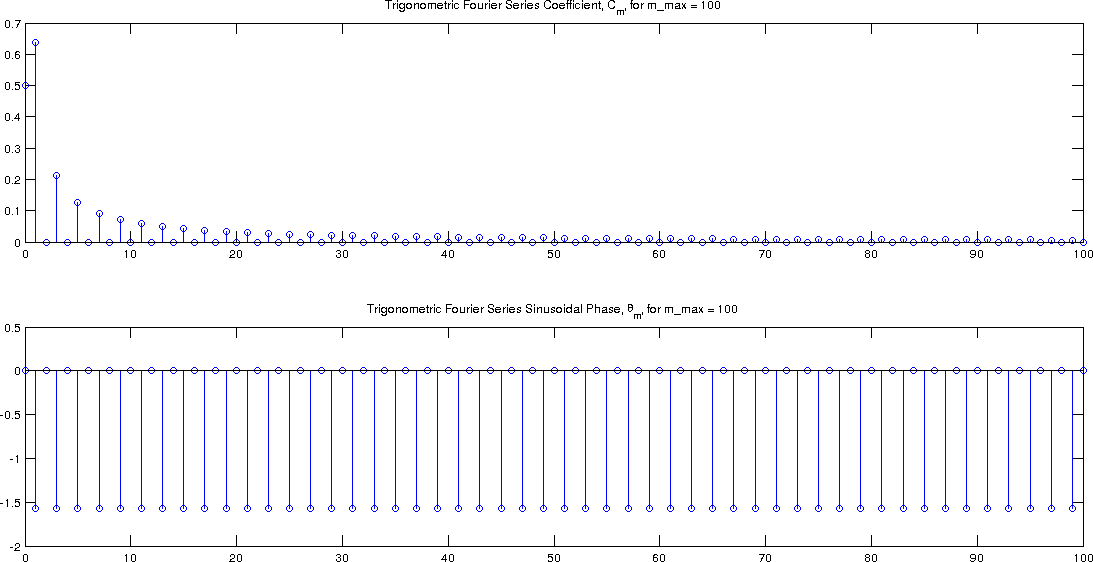
\includegraphics[width=0.70\textwidth]{images/ex2_2_1_cm_tm.png}
	\captionof{figure}{Trigonometric Fourier Series coefficients, $C_m$, and sinusoidal phase, $\theta_m$, for $m\_max = 100$}
	\label{fig:ex2_2_1_cm_tm}
\end{center}

\noindent Abaixo seguem as aproximações sucessivas do sinal através da Série de Fourier para $m \in [0, 1, 3, 5, 10, 50 e 100]$.
\begin{center}
	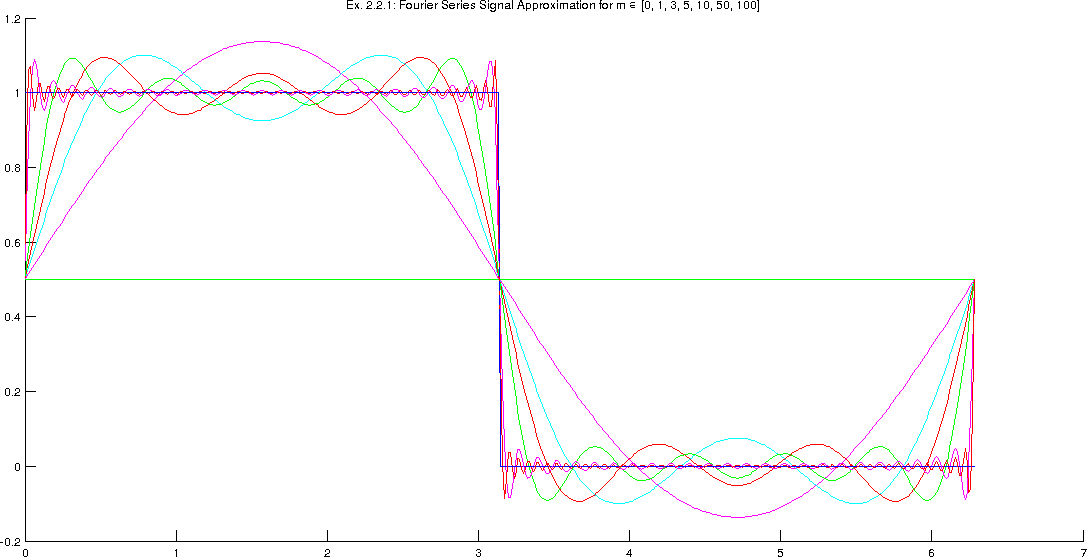
\includegraphics[width=0.70\textwidth]{images/ex2_2_1_approx.png}
	\captionof{figure}{Fourier Series Signal Approximation for $m\in [0, 1, 3, 5, 10, 50, 100]$}
	\label{fig:ex2_2_1_approx}
\end{center}

\noindent Abaixo apresentam-se a amplitude e fase dos valores dos coeficientes da Série de Fourier Complexa, $c_m$, para $m \in [-100, 100]$, obtidos a partir dos valores de $C_m$ e $\theta_m$ da correspondente Série de Fourier Trigonométrica.
\begin{center}
	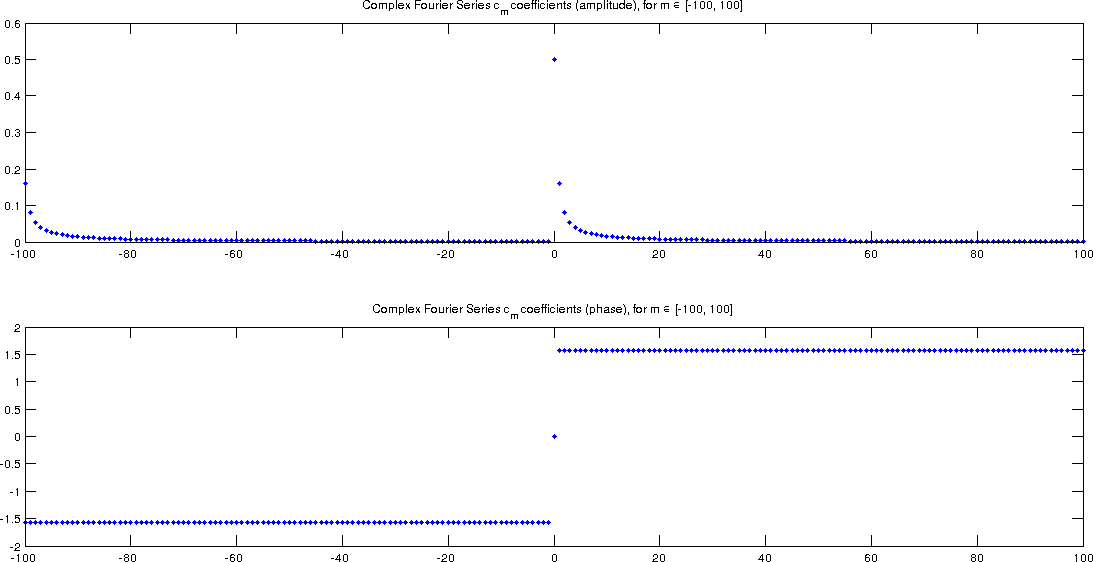
\includegraphics[width=0.70\textwidth]{images/ex2_2_1_complex_cm.png}
	\captionof{figure}{Complex Fourier Series $c_m$ coefficients for $m \in [-100, 100]$, represented in amplitude (above) and phase (below).}
	\label{fig:ex2_2_1_complex_cm}
\end{center}

\subsubsection{Exercise 2.2.2}
\noindent Apresentam-se de seguida os coeficientes da Série de Fourier Trigonométrica, $C_m$, bem como as fases, $\theta_m$, para uma \textbf{onda em dente de serra de período} $\mathbf{2 \pi s}$, para $m$ máximo de $100$.

\begin{center}
	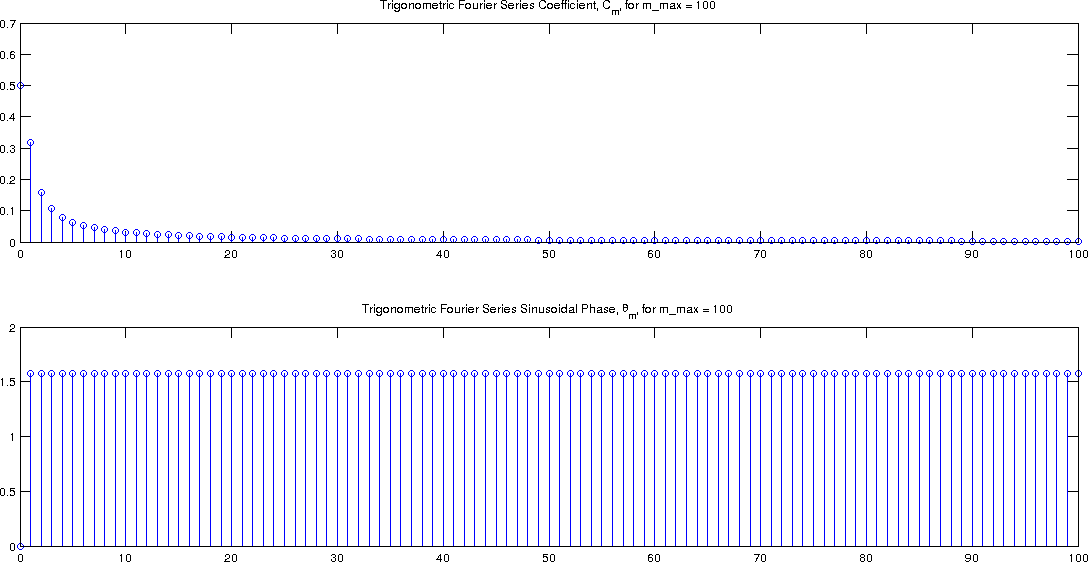
\includegraphics[width=0.70\textwidth]{images/ex2_2_2_cm_tm.png}
	\captionof{figure}{Trigonometric Fourier Series coefficients, $C_m$, and sinusoidal phase, $\theta_m$, for $m\_max = 100$}
	\label{fig:ex2_2_2_cm_tm}
\end{center}

\noindent Abaixo seguem as aproximações sucessivas do sinal através da Série de Fourier para $m \in [0, 1, 3, 5, 10, 50, 100]$.
\begin{center}
	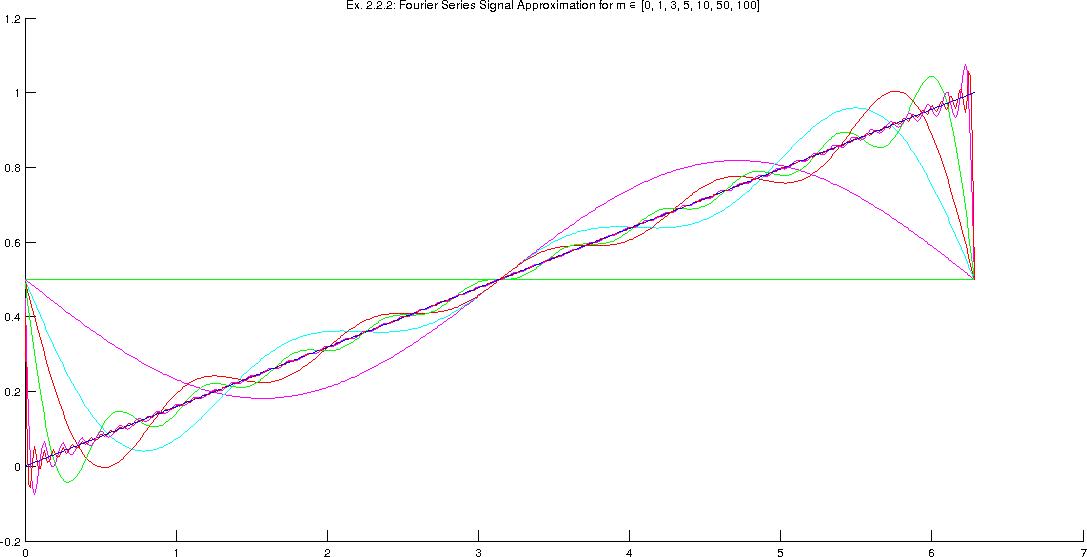
\includegraphics[width=0.70\textwidth]{images/ex2_2_2_approx.png}
	\captionof{figure}{Fourier Series Signal Approximation for $m\in [0, 1, 3, 5, 10, 50, 100]$}
	\label{fig:ex2_2_2_approx}
\end{center}

\noindent Abaixo apresentam-se a amplitude e fase dos valores dos coeficientes da Série de Fourier Complexa, $c_m$, para $m \in [-100, 100]$, obtidos a partir dos valores de $C_m$ e $\theta_m$ da correspondente Série de Fourier Trigonométrica.
\begin{center}
	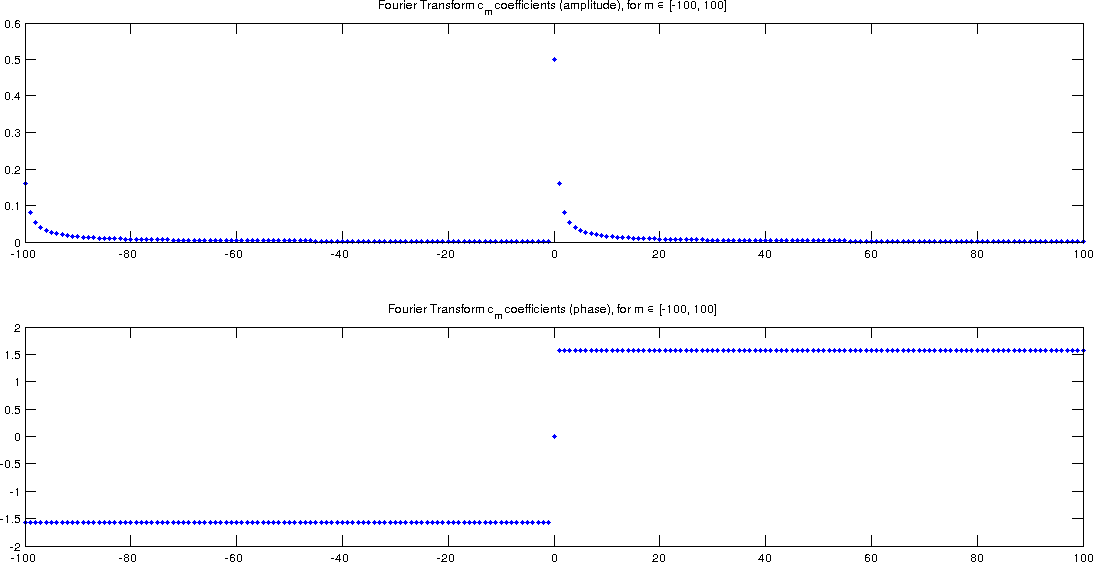
\includegraphics[width=0.70\textwidth]{images/ex2_2_2_complex_cm.png}
	\captionof{figure}{Complex Fourier Series $c_m$ coefficients for $m \in [-100, 100]$, represented in amplitude (above) and phase (below).}
	\label{fig:ex2_2_2_complex_cm}
\end{center}

\subsubsection{Exercise 2.2.3}
\label{subsubsec:ex_2_2_3}
\noindent Apresentam-se de seguida os coeficientes da Série de Fourier Trigonométrica, $C_m$, bem como as fases, $\theta_m$, para o sinal
\[
	x(t) = 1 + 2 \, sin\left(12 \, \pi \, t + \frac{\pi}{4}\right) \, cos(21 \, \pi \, t)
\]

\noindent para $m$ máximo de $100$. Após a simplificação da expressão (ver \emph{\nameref{subsec:ex_2_3}}), i. e.
\[
	x(t) = cos(0) + cos\left(33 \, \pi \, t + \frac{7 \pi}{4}\right) + cos\left(9 \, \pi \, t + \frac{\pi}{4}\right)
\]

\noindent é possível concluir que o período fundamental da função é $\frac{2}{3} \, s$ (já que a frequência angular fundamental é $3 \, \pi \, rad/s$).

\begin{center}
	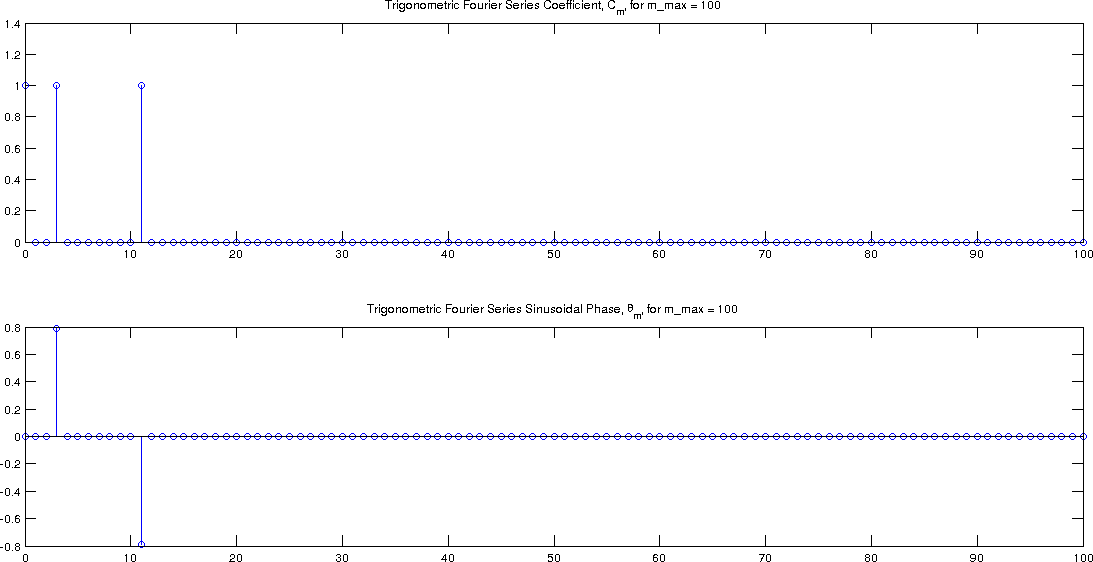
\includegraphics[width=0.70\textwidth]{images/ex2_2_3_cm_tm.png}
	\captionof{figure}{Trigonometric Fourier Series coefficients, $C_m$, and sinusoidal phase, $\theta_m$, for $m\_max = 100$}
	\label{fig:ex2_2_3_cm_tm}
\end{center}

\noindent Abaixo seguem as aproximações sucessivas do sinal através da Série de Fourier para $m \in [0, 1, 3, 5, 10, 50, 100]$.
\begin{center}
	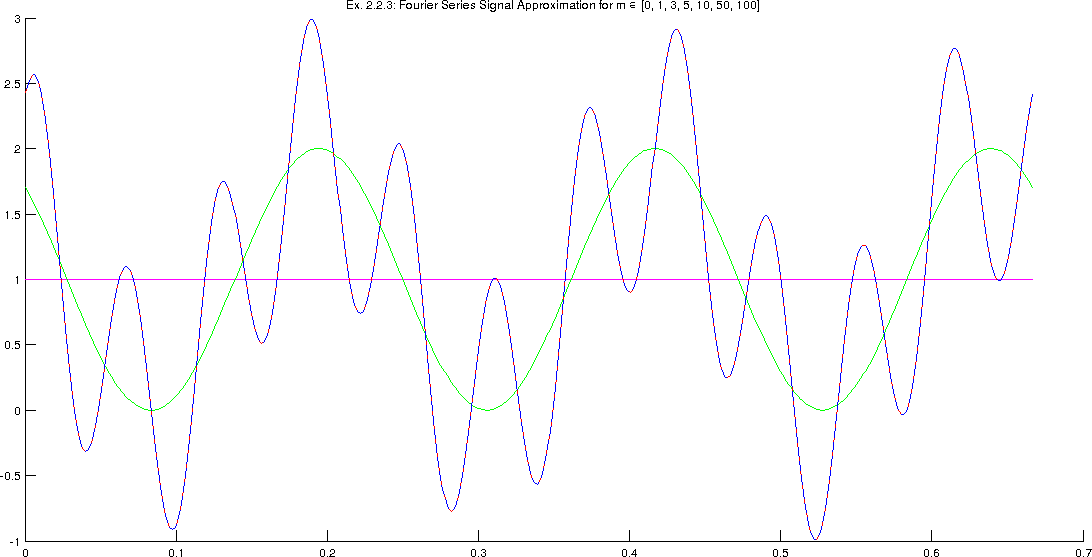
\includegraphics[width=0.70\textwidth]{images/ex2_2_3_approx.png}
	\captionof{figure}{Fourier Series Signal Approximation for $m\in [0, 1, 3, 5, 10, 50, 100]$}
	\label{fig:ex2_2_3_approx}
\end{center}

\noindent Abaixo apresentam-se a amplitude e fase dos valores dos coeficientes da Série de Fourier Complexa, $c_m$, para $m \in [-100, 100]$, obtidos a partir dos valores de $C_m$ e $\theta_m$ da correspondente Série de Fourier Trigonométrica.
\begin{center}
	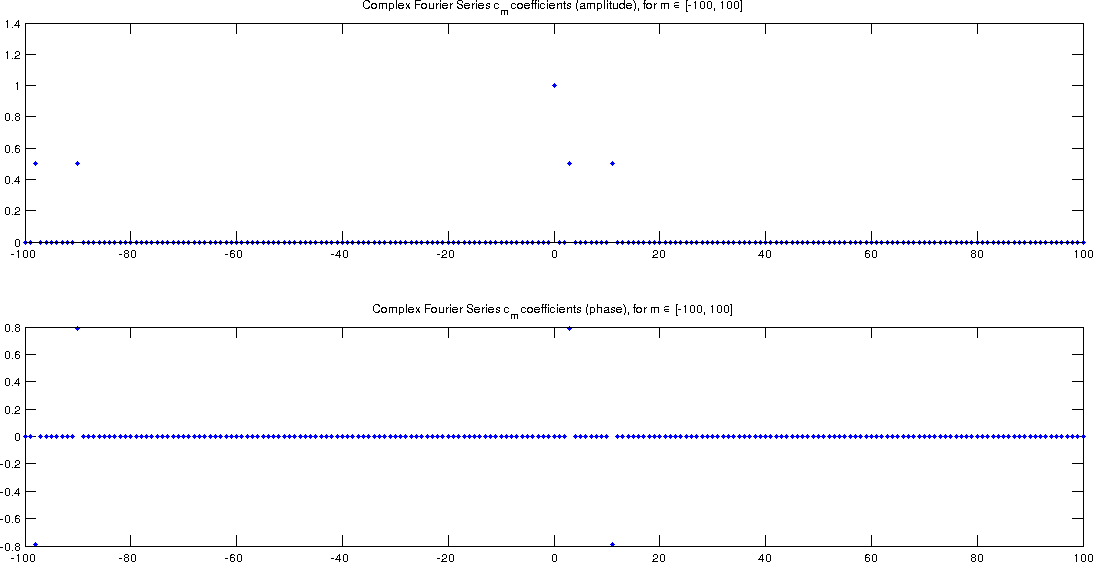
\includegraphics[width=0.70\textwidth]{images/ex2_2_3_complex_cm.png}
	\captionof{figure}{Complex Fourier Series $c_m$ coefficients for $m \in [-100, 100]$, represented in amplitude (above) and phase (below).}
	\label{fig:ex2_2_3_complex_cm}
\end{center}

\subsubsection{Exercise 2.2.4}
\label{subsubsec:ex_2_2_4}
\noindent Apresentam-se de seguida os coeficientes da Série de Fourier Trigonométrica, $C_m$, bem como as fases, $\theta_m$, para o sinal
\[
	x(t) = -2 + 4 \, cos\left(4 \, t + \frac{\pi}{3}\right) - 2 \, sin(10 \, t)
\]

\noindent para $m$ máximo de $100$. Após a simplificação da expressão (ver \emph{\nameref{subsec:ex_2_3}}), i. e.
\[
	x(t) = 2 \, cos(\pi) + 4 \, cos\left(4 \, t + \frac{\pi}{3}\right) + 2 \, cos\left(10 \, t + \frac{\pi}{2}\right)
\]

\noindent é possível concluir que o período fundamental da função é $\pi \, s$ (já que a frequência angular fundamental é $2 \, rad/s$).

\begin{center}
	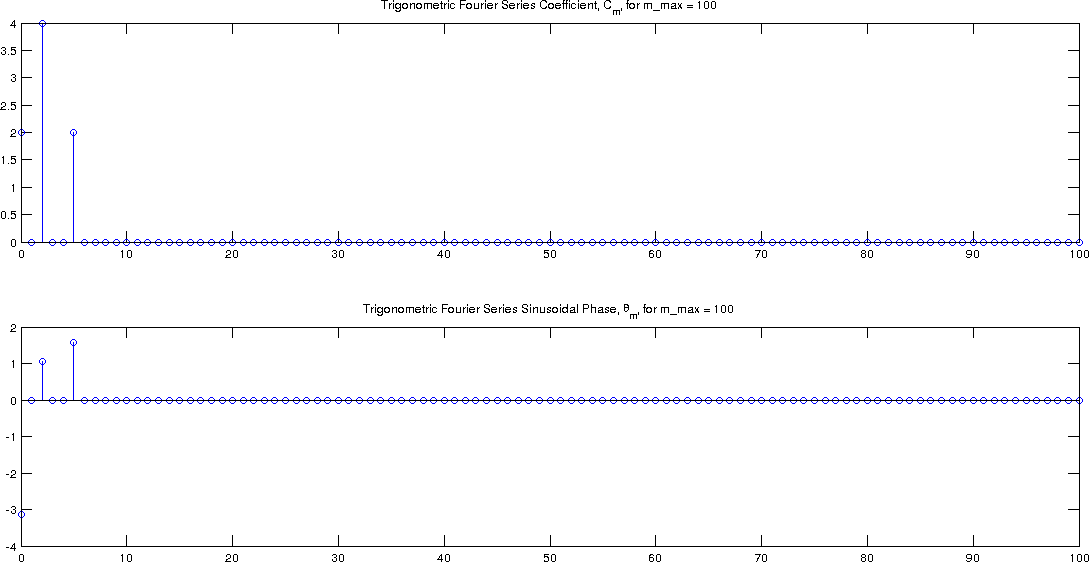
\includegraphics[width=0.70\textwidth]{images/ex2_2_4_cm_tm.png}
	\captionof{figure}{Trigonometric Fourier Series coefficients, $C_m$, and sinusoidal phase, $\theta_m$, for $m\_max = 100$}
	\label{fig:ex2_2_4_cm_tm}
\end{center}

\noindent Abaixo seguem as aproximações sucessivas do sinal através da Série de Fourier para $m \in [0, 1, 3, 5, 10, 50, 100]$.
\begin{center}
	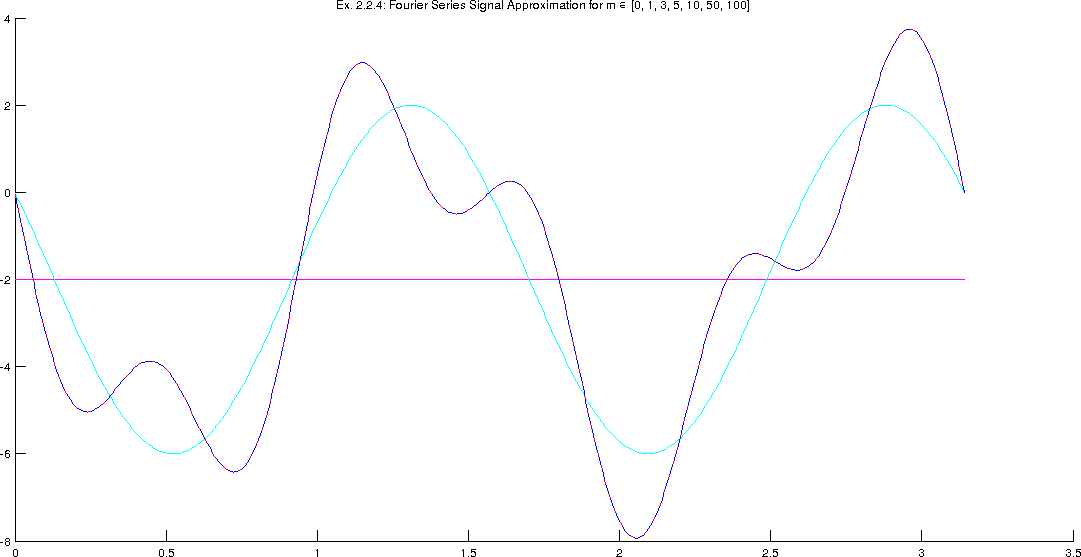
\includegraphics[width=0.70\textwidth]{images/ex2_2_4_approx.png}
	\captionof{figure}{Fourier Series Signal Approximation for $m\in [0, 1, 3, 5, 10, 50, 100]$}
	\label{fig:ex2_2_4_approx}
\end{center}

\noindent Abaixo apresentam-se a amplitude e fase dos valores dos coeficientes da Série de Fourier Complexa, $c_m$, para $m \in [-100, 100]$, obtidos a partir dos valores de $C_m$ e $\theta_m$ da correspondente Série de Fourier Trigonométrica.
\begin{center}
	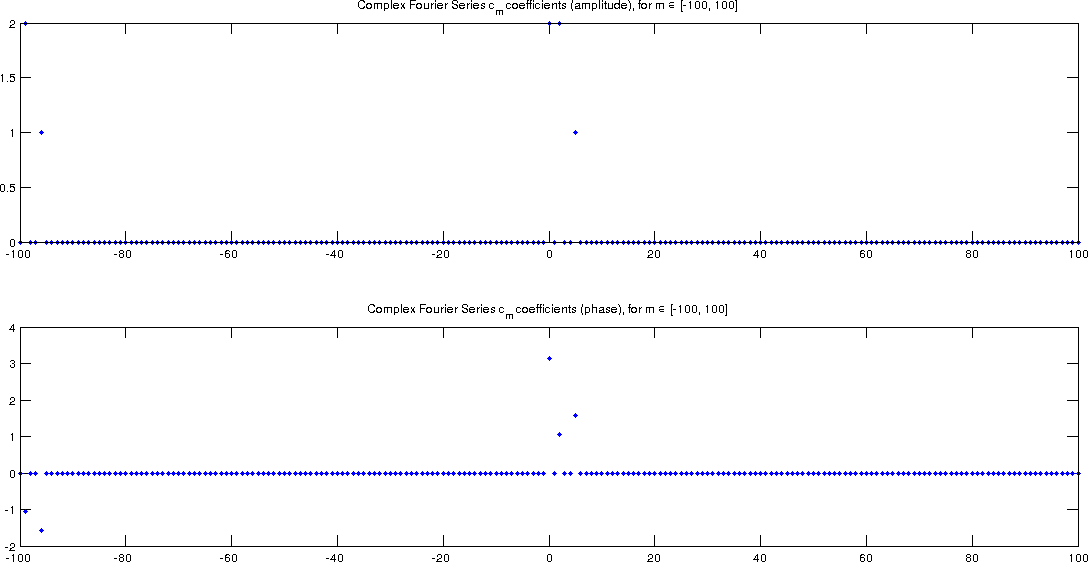
\includegraphics[width=0.70\textwidth]{images/ex2_2_4_complex_cm.png}
	\captionof{figure}{Complex Fourier Series $c_m$ coefficients for $m \in [-100, 100]$, represented in amplitude (above) and phase (below).}
	\label{fig:ex2_2_4_complex_cm}
\end{center}

\subsection{Exercise 2.3}
\noindent Para obter os coeficientes não-nulos da Série de Fourier Trigonométrica é útil analisar a expressão do sinal simplificada, isto é, segundo a forma
\begin{equation}
x_{1}(t) = \sum_{i} C_{i} \, cos(\omega_{i} t + \theta_{i})
\end{equation}

\subsubsection{\nameref{subsubsec:ex_2_2_3} Analysis}
\noindent Apresenta-se a simplificação da expressão da alínea \emph{\nameref{subsubsec:ex_2_2_3}}.
\begin{eqnarray}
	x(t) & = & 1 + 2 \, sin\left(12 \, \pi \, t + \frac{\pi}{4}\right) \, cos(21 \, \pi \, t) \\
	& = & 1 + sin\left(12 \, \pi \, t + \frac{\pi}{4} + 21 \, \pi \, t\right) + sin\left(12 \, \pi \, t + \frac{\pi}{4} - 21 \, \pi \, t\right) \\
	& = & 1 + sin\left(33 \, \pi \, t + \frac{\pi}{4}\right) + sin\left(-9 \, \pi \, t + \frac{\pi}{4}\right) \\
	& = & 1 + cos\left(\frac{\pi}{2} - \left(33 \, \pi \, t + \frac{\pi}{4}\right)\right) + cos\left(\frac{\pi}{2} - \left(-9 \, \pi \, t + \frac{\pi}{4}\right)\right) \\
	& = & 1 + cos\left(- 33 \, \pi \, t + \frac{\pi}{4}\right) + cos\left(9 \, \pi \, t + \frac{\pi}{4}\right) \\
	& = & cos(0) + cos\left(9 \, \pi \, t + \frac{\pi}{4}\right) + cos\left(33 \, \pi \, t + \frac{7 \, \pi}{4}\right)
\end{eqnarray}

\noindent A frequência fundamental é o máximo divisor comum entre as várias frequências angulares. Dado que a frequência angular designa $\omega$ numa expressão do tipo $cos(\omega \, t + \theta)$, a frequência fundamental será
\begin{equation}
	w_0 = gcd(0, 9 \pi, 33 \pi) = 3 \pi
\end{equation}

\noindent Obtém-se a partir dela o período fundamental (utilizado na alínea anterior para o \emph{plotting}).
\begin{equation}
	T_0 = \frac{2 \pi}{w_0} = \frac{2 \pi}{3 \pi} = \frac{2}{3} \, s
\end{equation}

\noindent Obtêm-se assim os coeficientes não-nulos da Série de Fourier: $\left[\frac{0}{3 \pi}, \frac{9 \pi}{3 \pi}, \frac{33 \pi}{3 \pi}\right] = [0, 3, 11]$.

\noindent A tabela final:

\begin{center}
	\begin{tabular}{|c|c|c|c|}
		\hline
		$\mathbf{m}$ & 0 & 3 & 11 \\
		\hline
		$\mathbf{C_m}$ & 1 & 1 & 1 \\
		\hline
		$\mathbf{\theta_m}$ & 0 & $\frac{\pi}{4}$ & $\frac{7 \pi}{4}$ \\
		\hline
	\end{tabular}
	\label{tab:ex_2_1_3}
\end{center}

\noindent Estes resultados são coerentes com a imagem (\ref{fig:ex2_2_3_cm_tm}) (considere-se que $cos\left(\frac{7 \pi}{4}\right) = cos\left(-\frac{\pi}{4}\right)$).

\subsubsection{\nameref{subsubsec:ex_2_2_4} Analysis}
\noindent Apresenta-se a simplificação da expressão da alínea \emph{\nameref{subsubsec:ex_2_2_4}}.
\begin{eqnarray}
	x(t) & = & -2 + 4 \, cos\left(4 \, t + \frac{\pi}{3}\right) - 2 \, sin(10 \, t) \\
	& = & -2 + 4 \, cos\left(4 \, t + \frac{\pi}{3}\right) - 2 \, cos\left(\frac{\pi}{2} - 10 \, t\right) \\
	& = & -2 + 4 \, cos\left(4 \, t + \frac{\pi}{3}\right) + 2 \, cos\left(\pi - \left(\frac{\pi}{2} - 10 \, t\right)\right) \\
	& = & 2 \, cos(\pi) + 4 \, cos\left(4 \, t + \frac{\pi}{3}\right) + 2 \, cos\left(10 \, t + \frac{\pi}{2}\right)
\end{eqnarray}

\noindent A frequência fundamental é o máximo divisor comum entre as várias frequências angulares. Dado que a frequência angular designa $\omega$ numa expressão do tipo $cos(\omega \, t + \theta)$, a frequência fundamental será
\begin{equation}
	w_0 = gcd(0, 4, 10) = 2
\end{equation}

\noindent Obtém-se a partir dela o período fundamental (utilizado na alínea anterior para o \emph{plotting}).
\begin{equation}
	T_0 = \frac{2 \pi}{w_0} = \frac{2 \pi}{2} = \pi \, s
\end{equation}

\noindent Obtêm-se assim os coeficientes não-nulos da Série de Fourier: $\left[\frac{0}{2}, \frac{4}{2}, \frac{10}{2}\right] = [0, 2, 5]$.

\noindent A tabela final:

\begin{center}
	\begin{tabular}{|c|c|c|c|}
		\hline
		$\mathbf{m}$ & 0 & 2 & 5 \\
		\hline
		$\mathbf{C_m}$ & 2 & 4 & 2 \\
		\hline
		$\mathbf{\theta_m}$ & $\pi$ & $\frac{\pi}{3}$ & $\frac{\pi}{2}$ \\
		\hline
	\end{tabular}
	\label{tab:ex_2_1_3}
\end{center}

\noindent Estes resultados são coerentes com a imagem (\ref{fig:ex2_2_4_cm_tm}) (considere-se que $cos(\pi) = cos(-\pi)$).

\section{Exercise 3}
\noindent TODO %%% TODO

\section{Exercise 4}
\noindent TODO %%% TODO

\section{Attachments}
\subsection{Trigonometric identities}
\label{subsec:trigident}
As simplicações das alíneas \emph{\nameref{subsubsec:ex_2_2_3}} e \emph{\nameref{subsubsec:ex_2_2_4}} fazem uso das seguintes igualdades:
\begin{equation}
sin(\theta) \, cos(\varphi) = \frac{cos(\theta - \varphi) + cos(\theta + \varphi)}{2}
\end{equation}

\begin{equation}
cos\left(\theta + \frac{\pi}{2}\right) = -sin(\theta)
\end{equation}

\begin{equation}
cos(\theta + \pi) = -cos(\theta)
\end{equation}

\begin{equation}
cos(-\theta) = cos(\theta)
\end{equation}

\end{document}
